
\chapter{Introduction and notation}
%\label{ch:intro}

\section{Basic sets}
%\label{sec:basic}

\noindent{\large \bf Exercises --- \thesection\ }

\begin{enumerate}

\item Each of the quantities indexing the rows of the following table
is in one or more of the sets which index the columns.  Place a 
check mark in a table entry if the quantity is in the set.

\begin{tabular}{|c||c|c|c|c|c|} \hline
 & $\Naturals$ & $\Integers$ & $\Rationals$ & $\Reals$ & $\Complexes$
 \\ \hline\hline
\rule{0pt}{15pt} $17$ & & & & & \\ \hline
\rule{0pt}{15pt} $\pi$ & & & & & \\ \hline
\rule{0pt}{15pt} $22/7$ & & & & & \\ \hline
\rule{0pt}{15pt} $-6$ & & & & & \\ \hline
\rule{0pt}{15pt} $e^0$ & & & & & \\ \hline
\rule{0pt}{15pt} $1+i$ & & & & & \\ \hline
\rule{0pt}{15pt} $\sqrt{3}$ & & & & & \\ \hline
\rule{0pt}{15pt} $i^2$ & & & & & \\  \hline
\end{tabular}

\hint{Note that these sets contain one another, so if %
you determine that a number is a natural number it is automatically %
an integer and a rational number and a real number and a complex number\ldots}

\vfill

\hintspagebreak
\workbookpagebreak

\item Write the set $\Integers$ of integers using a singly infinite
listing.

\twsvspace{.25in}{1in}{.15in}

\hint{What the heck is meant by a ``singly infinite listing''?  To help you figure this out, note that 
\[ \ldots -3, -2, -1, 0, 1, 2, 3, \ldots \] 
\noindent is a doubly infinite listing.}

\vfill


\item Identify each as rational or irrational.
\begin{enumerate}
\item $5021.2121212121\ldots$
\item $0.2340000000\ldots$
\item $12.31331133311133331111\ldots$
\item $\pi$
\item $2.987654321987654321987654321\ldots$
\end{enumerate}

\vfill

\hint{rat,rat,irr,irr,rat}

\vfill

\textbookpagebreak

\item The ``see and say'' sequence is produced by first writing a 1, 
then iterating the following procedure:  look at the previous entry 
and say how many entries there are of each integer and write down what 
you just said.  The first several terms of the ``see and say'' sequence 
are $1, 11, 21, 1112, 3112, 211213, 312213, 212223, \ldots$.  Comment on the
rationality (or irrationality) of the number whose decimal digits are obtained 
by concatenating the ``see and say'' sequence.

\[ 0.1112111123112211213... \]

\vfill

\hint{
Experiment!

What would it mean for this number to be rational?  If we were to
run into an element of the ``see and say'' sequence that is its own description, then
from that point onward the sequence would get stuck repeating the same thing over and over
(and the number whose digits are found by concatenating the elements of the ``see and say'' 
sequence will enter into a repeating pattern.)
} 
\vfill

\workbookpagebreak

\item Give a description of the set of rational numbers whose decimal
expansions terminate.  (Alternatively, you may think of their decimal
expansions ending in an infinitely-long string of zeros.)

\hint{If a decimal expansion terminates after, say, k digits, can you figure out how to produce an integer from that number? Think about multiplying by something \ldots}

\vfill

\item Find the first 20 decimal places of $\pi$, $3/7$, $\sqrt{2}$, 
  $2/5$, $16/17$, $\sqrt{3}$, $1/2$ and $42/100$.  Classify each of
these quantity's decimal expansion as: terminating, having a repeating
pattern, or showing no discernible pattern.

\hint{A calculator will generally be inadequate for this problem. You should try using a CAS (Computer Algebra System).  I  would recommend the Sage computer algebra system because
like this book it is free -- you can download sage and run it on your own system or you can try it out online without installing.  Check it out at www.sagemath.org.

You can get sage to output $\pi$ to high accuracy by typing {\tt pi.N(digits=21)}
at the sage$>$ prompt.}

\vfill

\workbookpagebreak
 
\item Consider the process of long division.  Does this algorithm give
any insight as to why rational numbers have terminating or repeating
decimal expansions?  Explain.

\hint{You really need to actually sit down and do some long division problems.  When in the process do you suddenly realize that the digits are going to repeat?  Must this decision point always occur? Why?}

\vfill

\item Give an argument as to why the product of two rational numbers
is again a rational.

\hint{Take for granted that the usual rule for multiplying two fractions is okay to use:

\[ \frac{a}{b} * \frac{c}{d} \; = \; \frac{ac}{bd}. \]

\noindent How do you know that the result is actually a rational number?}

\vfill

\textbookpagebreak

\hintspagebreak

\item Perform the following computations with complex numbers

  \begin{enumerate}
  \item \rule{0pt}{20pt}$ (4 + 3i) - (3 + 2i) $
  \item \rule{0pt}{20pt}$ (1 + i) + (1 - i) $
  \item \rule{0pt}{20pt}$ (1 + i) \cdot (1 - i) $
  \item \rule{0pt}{20pt}$ (2 - 3i) \cdot (3 - 2i) $
  \end{enumerate}

\hint{These are straightforward. If you really must verify these somehow, you can go to a CAS like Sage, or you can learn how to enter complex numbers on your graphing calculator. (On my TI-84, you get i by hitting the 2nd key and then the decimal point.)
}

\item The {\em conjugate} of a complex number is denoted with a
  superscript star, and is formed by negating the imaginary part.
  Thus if $z = 3+ 4i$ then the conjugate of $z$ is  $z^\ast = 3-4i$.
  Give an argument as to why the product of a complex number and its
  conjugate is a real quantity.  (I.e. the imaginary part of
  $z\cdot z^\ast$ is necessarily 0, no matter what complex number is
  used for $z$.) 

\hint{This is really easy, but be sure to do it generically. In other words, don't just use examples -- do the calculation with variables for the real and imaginary parts of the complex number.
}

\vfill

\workbookpagebreak

\end{enumerate}



%% Emacs customization
%% 
%% Local Variables: ***
%% TeX-master: "GIAM.tex" ***
%% comment-column:0 ***
%% comment-start: "%% "  ***
%% comment-end:"***" ***
%% End: ***


\newpage

\section{Definitions: Prime numbers}
%\label{sec:def}

\noindent{\large\bf Exercises --- \thesection\ }

\begin{enumerate}

\item Find the prime factorizations of the following integers.

  \begin{enumerate}
  \item 105
  \item 414
  \item 168
  \item 1612
  \item 9177
  \end{enumerate}

\hint{Divide out the obvious factors in order to reduce the complexity of the remaining problem. The first number is divisible by 5. The next three are all even. Recall that a number is divisible by 3 if and only if the sum of its digits is divisible by 3.
}

\item Use the sieve of Eratosthenes to find all prime numbers
up to 100.

\begin{tabular}{cccccccccc}
\rule{14pt}{0pt} & \rule{14pt}{0pt} & \rule{14pt}{0pt} &
\rule{14pt}{0pt} & \rule{14pt}{0pt} & \rule{14pt}{0pt} & 
\rule{14pt}{0pt} & \rule{14pt}{0pt} & \rule{14pt}{0pt} &
\rule{14pt}{0pt} \\
 1 & 2 & 3 & 4 & 5 & 6 & 7 & 8 & 9 & 10 \\
 11 & 12 & 13 & 14 & 15 & 16 & 17 & 18 & 19 & 20 \\
 21 & 22 & 23 & 24 & 25 & 26 & 27 & 28 & 29 & 30 \\
 31 & 32 & 33 & 34 & 35 & 36 & 37 & 38 & 39 & 40 \\
 41 & 42 & 43 & 44 & 45 & 46 & 47 & 48 & 49 & 50 \\
 51 & 52 & 53 & 54 & 55 & 56 & 57 & 58 & 59 & 60 \\ 
 61 & 62 & 63 & 64 & 65 & 66 & 67 & 68 & 69 & 70 \\
 71 & 72 & 73 & 74 & 75 & 76 & 77 & 78 & 79 & 80 \\
 81 & 82 & 83 & 84 & 85 & 86 & 87 & 88 & 89 & 90 \\
 91 & 92 & 93 & 94 & 95 & 96 & 97 & 98 & 99 & 100
\end{tabular}

\hint{The primes used in this instance of the sieve are just 2, 3, 5 and 7. Any number less than 100 that isn't a multiple of 2, 3, 5 or 7 will not be crossed off during the sieving process. If you're still unclear about the process, try a web search for {\tt "Sieve of Eratosthenes" +applet}, there are several interactive applets that will help you to understand how to sieve.
}

\item What would be the largest prime one would sieve with
in order to find all primes up to 400?

\hint{Remember that if a number factors into two multiplicands, the smaller of them will be less than the square root of the original number.}

\wbvfill

\workbookpagebreak

\item Characterize the prime factorizations of numbers that are
  perfect squares.

\wbvfill

\hint{It might be helpful to write down a bunch of examples. Think about how the prime factorization of a number gets transformed when we square it.}

\textbookpagebreak

\item Complete the following table which is related to 
\ifthenelse{\boolean{InTextBook}}{Conjecture~\ref{conj:ferm}}{the conjecture that whenever $p$ is a prime number, $2^p-1$ is also a prime}.

\begin{tabular}{c|c|c|c}
$p$ & $2^p-1$ & prime? & factors \\ \hline
2 & 3 & yes & 1 and 3 \\
3 & 7 & yes & 1 and 7 \\
5 & 31 & yes &  \\
7 & 127   &     &    \\
11 &   &     &    
\end{tabular}

\hint{
You'll need to determine if $2^{11}-1 = 2047$ is prime or not. If you never figured out how to read the table of primes on page 15, here's a hint: If 2047 was a prime there would be a 7 in the cell at row 20, column 4.

A quick way to find the factors of a not-too-large number is to use the "table" feature of your graphing calculator. If you enter y1=2047/X and select the table view (2ND GRAPH). Now, just scan down the entries until you find one with nothing after the decimal point. That's an X that evenly divides 2047!

An even quicker way is to type {\tt factor(2047)} in Sage.
}



\hintspagebreak

\item Find a counterexample for \ifthenelse{\boolean{InTextBook}}{Conjecture~\ref{conj:poly}}{the conjecture that $x^2-31x+257$ evaluates to a prime number
whenever $x$ is a natural number}.

\wbvfill

\hint{Part of what makes the "prime-producing-power" of that polynomial impressive is that it gives each prime twice -- once on the descending arm of the parabola and once on the ascending arm. In other words, the polynomial gives prime values on a set of contiguous natural numbers {0,1,2, ..., N} and the vertex of the parabola that is its graph lies dead in the middle of that range. You can figure out what N is by thinking about the other end of the range: (-1)2 + 31 · (-1) + 257 = 289 (289 is not a prime, you should recognize it as a perfect square.)}

\item Use the second definition of ``prime'' to see that $6$ is
not a prime.  In other words, find two numbers (the $a$ and $b$ 
that appear in the definition) such that $6$ is not a factor of
either, but {\em is} a factor of their product.

\wbvfill

\hint{Well, we know that 6 really isn't a prime... Maybe its factors enter into this somehow\ldots}

\item Use the second definition of ``prime'' to show that $35$ is
not a prime.

\wbvfill

\hint{How about $a=2\cdot5$ and $b=3\cdot7$.  Now you come up with a different pair!}

\workbookpagebreak

\item A famous conjecture that is thought to be true (but
for which no proof is known) is the  \index{Twin Prime conjecture}
Twin Prime conjecture.
A pair of primes is said to be twin if they differ by 2.
For example, 11 and 13 are twin primes, as are 431 and 433.
The Twin Prime conjecture states that there are an infinite
number of such twins.  Try to come up with an argument as
to why 3, 5 and 7 are the only prime triplets.

\wbvfill

\hint{It has to do with one of the numbers being divisible by 3. (Why is this forced to be the case?) If that number isn't actually 3, then you know it's composite.}



\item Another famous conjecture, also thought to be true -- but
as yet unproved, is \index{Goldbach's conjecture}
Goldbach's conjecture.  Goldbach's conjecture
states that every even number greater than 4 is the sum of two odd
primes.  There is a function $g(n)$, known as the Goldbach function, defined
on the positive integers, that gives the number of different ways to 
write a given number as the sum of two odd primes.  For example $g(10) = 2$
since $10=5+5=7+3$.  Thus another version of Goldbach's conjecture
is that $g(n)$ is positive whenever $n$ is an even number greater than
4.

Graph $g(n)$ for $6 \leq n \leq 20$.

\wbvfill

\hint{If you don't like making graphs, a table of the values of g(n) would suffice. Note that we don't count sums twice that only differ by order. For example, 16 = 13+3 and 11+5 (and 5+11 and 3+13) but g(16)=2.}

\end{enumerate}

\newpage

\section{More scary notation}
%\label{sec:scary}

\noindent{\large\bf Exercises --- \thesection\ }

\begin{enumerate}

\item How many quantifiers (and what sorts) are in the following sentence?

``Everybody has \emph{some} friend that thinks they know everything about 
a sport.''
  
\wbvfill

\hint{Four.}

\item The sentence ``Every metallic element is a solid at room temperature.'' 
is false.  Why?

\wbvfill

\hint{The chemical symbol for an element that is an exception is Hg which stands for "Hydro-argyrum" it is also known as "liquid silver" or "quick silver".}

\item The sentence ``For every pair of (distinct) real numbers there is 
another real number between them.'' is true.  Why?

\wbvfill

\hint{Think about this: is there any way to (using a formula) find a number that lies in between two other numbers?}

\item Write your own sentences containing four quantifiers.  One
sentence in which the quantifiers appear ($\forall \exists \forall \exists$)
and another in which they appear ($\exists \forall \exists \forall$).

\wbvfill

\hint{You're on your own here. Be inventive!}

\end{enumerate}


\newpage


\section{Definitions of elementary number theory}
%\label{sec:num_thry}

\noindent{\large\bf Exercises --- \thesection\ }

\begin{enumerate}

\item An integer $n$ is \index{doubly-even} \emph{doubly-even} 
if it is even, and the integer $m$ guaranteed to exist because 
$n$ is even is itself even.  Is 0 doubly-even?  What are the 
first 3 positive, doubly-even integers?

\wbvfill

\hint{Answers: yes, 0,4 and 8.}

\item Dividing an integer by two has an interesting interpretation
when using binary notation: simply shift the digits to the right.
Thus, $22 = 10110_2$ when divided by two gives $1011_2$ which is
$8+2+1=11$.  How can you recognize a doubly-even integer from
its binary representation?

\wbvfill

\hint{Even numbers have a zero in their units place. What digit must also be zero in a doubly-even number's binary representation?}

\item The \index{octal representation} \emph{octal} representation 
of an integer uses powers of 8 in place notation.  The digits of an 
octal number run from 0 to 7, one never sees 8's or 9's.  How would 
you represent 8 and 9 as octal numbers?  What octal number comes 
immediately after $777_8$?  What (decimal) number is $777_8$?

\wbvfill

\workbookpagebreak

\hint{Eight is $10_8$, nine is $11_8$. The point of asking questions about $777$, is that (in octal) $7$ is the digit that is analogous to $9$ in base-$10$. Thus $777_8$ is something like $999_{10}$ in that the number following both of them is written $1000$ (although $1000_8$ and $1000_{10}$ are certainly not equal!)}

\hintspagebreak

\item One method of converting from decimal to some other base is
called \index{repeated division algorithm} \emph{repeated division}.  
One divides the number by the base
and records the remainder -- one then divides the quotient obtained
by the base and records the remainder.  Continue dividing the 
successive quotients by the base until the quotient is smaller than
the base.  Convert 3267 to base-7 using repeated division.  Check 
your answer by using the meaning of base-7 place notation.  (For
example $54321_7$ means $5\cdot7^4 + 4\cdot7^3 + 3 \cdot7^2 +
2\cdot7^1 + 1\cdot7^0$.)

\wbvfill

\hint{It is helpful to write something of the form $n = qd+r$ at each stage. The first two stages should look like

\[ 3267 \; = \; 466 \cdot 7 + 5 \]

\[ 466 \; = \; 66 \cdot 7 + 4 \]

you do the rest\ldots
}

\item State a theorem about the octal representation of even numbers.

\wbvfill

\hint{One possibility is to mimic the result for base-10 that an even number always ends in 0,2,4,6 or 8.}

\item In hexadecimal (base-16) notation one needs 16 ``digits,'' the
  ordinary digits are used for 0 through 9, and the letters A through
  F are used to give single symbols for 10 through 15.  The first  32
  natural number in hexadecimal are:
  1,2,3,4,5,6,7,8,9,A,B,C,D,E,F,10,11,12,13,14,15,16,\newline 17,18,19,1A,
  1B,1C,1D,1E,1F,20. 

  Write the next 10 hexadecimal numbers after $AB$.

  Write the next 10 hexadecimal numbers after $FA$.

\hint{As a check, the tenth number after AB is B5.\newline
The tenth hexadecimal number after FA is 104.}

\wbvfill

\workbookpagebreak

\item For conversion between the three bases used most often in 
Computer Science we can take binary as the ``standard'' base and 
convert using a table look-up.  Each octal digit will correspond 
to a binary triple, and each hexadecimal digit will correspond to 
a 4-tuple of binary numbers.  Complete the following tables.  
(As a check, the 4-tuple next to $A$ in the table for
hexadecimal should be 1010 -- which is nice since $A$ 
is really 10 so if you read that as ``ten-ten'' it is a good 
aid to memory.)

\begin{center}
\begin{tabular}{ccc}
\begin{tabular}{|c|c|} \hline
octal & binary \\ \hline \hline
\rule{0pt}{14pt} 0 & 000 \\ \hline
\rule{0pt}{14pt} 1 & 001 \\ \hline
\rule{0pt}{14pt} 2 & \\ \hline
\rule{0pt}{14pt} 3 & \\ \hline
\rule{0pt}{14pt} 4 & \\ \hline
\rule{0pt}{14pt} 5 & \\ \hline
\rule{0pt}{14pt} 6 & \\ \hline
\rule{0pt}{14pt} 7 & \\ \hline
\end{tabular}
 & \rule{72pt}{0pt} &
\begin{tabular}{|c|c|} \hline
hexadecimal & binary \\ \hline \hline
\rule{0pt}{14pt} 0 & 0000 \\ \hline
\rule{0pt}{14pt} 1 & 0001 \\ \hline
\rule{0pt}{14pt} 2 & 0010 \\ \hline
\rule{0pt}{14pt} 3 & \\ \hline
\rule{0pt}{14pt} 4 & \\ \hline
\rule{0pt}{14pt} 5 & \\ \hline
\rule{0pt}{14pt} 6 & \\ \hline
\rule{0pt}{14pt} 7 & \\ \hline
\rule{0pt}{14pt} 8 & \\ \hline
\rule{0pt}{14pt} 9 & \\ \hline
\rule{0pt}{14pt} A & \\ \hline
\rule{0pt}{14pt} B & \\ \hline
\rule{0pt}{14pt} C & \\ \hline
\rule{0pt}{14pt} D & \\ \hline
\rule{0pt}{14pt} E & \\ \hline
\rule{0pt}{14pt} F & \\ \hline
\end{tabular}
\end{tabular}
\end{center}
 
\hint{

\vfill

This is just counting in binary. Remember the sanity check that the hexadecimal digit A is represented by 1010 in binary.  ($10_{10} \; = \; A_{16} \; = \; 1010_{2}$)

\vfill

}

\hintspagebreak
\workbookpagebreak
\textbookpagebreak

\item Use the tables from the previous problem to make the following conversions.

\begin{enumerate}
\item Convert $757_8$ to binary.
\item Convert $1007_8$ to hexadecimal.
\item Convert $100101010110_2$ to octal.
\item Convert $1111101000110101_2$ to hexadecimal.
\item Convert $FEED_{16}$ to binary.
\item Convert $FFFFFF_{16}$ to octal.
\end{enumerate}

\hint{Answers for the first three:
\[  757_8 = 111 101 111_2 \]
\[ 1007_8 = 001 000 000 111_2 = 0010 0000 0111_2 = 207_{16} \]
\[ 100 101 010 110_2 = 4526_8 \]
}

\item Try the following conversions between various number systems:

\begin{enumerate}
\item Convert $30$ (base 10) to binary.
\item Convert $69$ (base 10) to base 5.
\item Convert $1222_3$ to binary.
\item Convert $1234_7$ to base 10.
\item Convert $EEED_{15}$ to base 12. (Use $\{1, 2, 3 \ldots 9, d, e\}$ as the digits in base 12.)
\item Convert $678_{9}$ to hexadecimal.
\end{enumerate}

\item It is a well known fact that if a number is divisible by 3, then 3
  divides the sum of the (decimal) digits of that number.  Is this
  result true in base 7?  Do you think this result is true in {\em
  any} base? 
 
 \wbvfill
 
\hint{Might this effect have something to do with 10 being just one bigger than 9 (a multiple of 3)?}

\item Suppose that 340 pounds of sand must be placed into bags having
  a 50 pound capacity.  Write an expression using either floor or
  ceiling notation for the number of bags required.

\wbvfill

\hint{Seven 50 pound bags would hold 350 pounds of sand. They'd also be able to handle 340 pounds!}

\item True or false? 

\[ \left\lfloor \frac{n}{d}\right\rfloor < \left\lceil \frac{n}{d}\right\rceil \]
 
\noindent for all integers $n$ and $d>0$. Support your claim.

\wbvfill

\hint{You have to try a bunch of examples.  You should try to make sure the examples
you try cover all the possibilities.  The pairs that provide counterexamples (i.e. show the statement is false in general) are relatively sparse, so be systematic.}

\workbookpagebreak

\item What is the value of $\lceil\pi\rceil^{2}-\lceil\pi^{2}\rceil$?

\wbvfill

\hint{ $\pi^2 = 9.8696$ }



\item Assuming the symbols $n$,$d$,$q$ and $r$ have meanings as in the
  quotient-remainder theorem (\ifthenelse{\boolean{InTextBook}}{Theorem~\ref{quo-rem} on page \pageref{quo-rem}}{see page 29 of GIAM}).  Write
  expressions for $q$ and $r$, in terms of $n$ and $d$ using floor
  and/or ceiling notation.

\wbvfill

\hint{I just can't bring myself to spoil this one for you, you really need to work this out on your own. }

\textbookpagebreak

\item Calculate the following quantities:

\begin{enumerate}
\item \wbitemsep $3 \mod 5$
\item \wbitemsep $37 \mod 7$
\item \wbitemsep $1000001 \mod 100000$
\item \wbitemsep $6 \tdiv 6$
\item \wbitemsep $7 \tdiv 6$
\item \wbitemsep $1000001 \tdiv 2$
\end{enumerate}

\hint{The even numbered ones are 2, 1, 500000.}

\hintspagebreak
\workbookpagebreak

\item Calculate the following binomial coefficients:

\begin{enumerate}
\item \wbitemsep $\binom{3}{0}$
\item \wbitemsep $\binom{7}{7}$
\item \wbitemsep $\binom{13}{5}$
\item \wbitemsep $\binom{13}{8}$
\item \wbitemsep $\binom{52}{7}$
\end{enumerate}

\hint{The even numbered ones are 1 and 1287. The TI-84 calculates binomial coefficients. The symbol used is {\tt nCr} (which is placed between the numbers -- i.e. it is an infix operator). You get {\tt nCr} as the 3rd item in the {\tt PRB} menu under {\tt MATH}. In sage the command is {\tt binomial(n,k)}.}

\item An ice cream shop sells the following flavors: chocolate, vanilla, 
strawberry, coffee, butter pecan, mint chocolate chip and raspberry.
How many different bowls of ice cream -- with three scoops -- can they make?  

\wbvfill

\hint{You're choosing three things out of a set of size seven\ldots}

\end{enumerate}


\newpage

\section[Some algorithms]{Some algorithms of elementary number theory}
%\label{sec:alg}

\noindent{\large\bf Exercises --- \thesection\ }

\begin{enumerate}

\item Trace through the division algorithm with inputs $n=27$ and
  $d=5$, each time an assignment statement is encountered write it
  out.  How many assignments are involved in this particular
  computation?
\hint{r=27 \newline
q=0  \newline
r=27-5=22  \newline
q=0+1=1  \newline
r=22-5=17  \newline
q=1+1=2  \newline
r=17-5=12  \newline
q=2+1=3  \newline
r=12-5=7  \newline
q=3+1=4  \newline
r=7-5=2  \newline
q=4+1=5  \newline
return r is 2 and q is 5.
}

\wbvfill

\item Find the gcd's and lcm's of the following pairs of numbers.
\medskip

\centerline{
\begin{tabular}{|c|c|c|c|} \hline
\rule[-3pt]{0pt}{18pt} $a$ & $b$ & $\gcd{a}{b}$ & $\lcm{a}{b}$ \\ \hline
\rule[-3pt]{0pt}{18pt} 110 & 273 & & \\ \hline
\rule[-3pt]{0pt}{18pt}105 & 42 & & \\ \hline
\rule[-3pt]{0pt}{18pt}168 & 189 & & \\ \hline
\end{tabular}
}

\hint{For such small numbers you can just find their prime factorizations and use that, although it might be useful to practice your understanding of the Euclidean algorithm by tracing through it to find the gcd's and then using the formula
\[ \lcm (a,b) = \frac{ab}{\gcd (a,b).} \]
}

\workbookpagebreak

\item Formulate a description of the gcd of two numbers in terms of
  their prime factorizations in the general case (when the
  factorizations may include powers of the primes involved).

\wbvfill

\hint{Suppose that one number's prime factorization contains $p^e$ and the other
contains $p^f$, where $e < f$. What power of $p$ will divide both, $p^e$ or $p^f$ ?}

\item Trace through the Euclidean algorithm with inputs $a=3731$ and
  $b=2730$, each time the assignment statement that calls the division
  algorithm is encountered write out the expression $a=qb+r$.   (With the
  actual values involved !) 

\wbvfill

\hint{The quotients you obtain should alternate between 1 and 2.}

\end{enumerate}


\newpage

\section{Rational and irrational numbers}
%\label{sec:rat}

\noindent{\large\bf Exercises --- \thesection\ }

\begin{enumerate}

\item \index{Rational approximation} Rational Approximation is 
a field of mathematics that has received much study.  The main idea 
is to find rational numbers that are very good approximations to
given irrationals.  For example, $22/7$ is a well-known rational 
approximation to $\pi$.  Find good rational approximations to 
$\sqrt{2}, \sqrt{3}, \sqrt{5}$ and $e$.

\vfill

\wbvfill

\hint{One approach is to truncate a decimal approximation and then rationalize. E.g. $\sqrt{2}$ is approximately 1.4142, so 14142/10000 isn't a bad approximator (although naturally 7071/5000 is better since it involves smaller numbers).}

\vfill

\item The theory of base-$n$ notation that we looked at in 
\ifthenelse{\boolean{InTextBook}}{sub-section~\ref{base-n}}{the sub-section on base-$n$} can be extended to deal with real and 
rational numbers by introducing a decimal point (which should 
probably be re-named in accordance with the base) and adding 
digits to the right of it.  For instance $1.1011$ is binary notation
for $1 \cdot 2^0 + 1 \cdot 2^{-1} + 0 \cdot 2^{-2} + 
1\cdot 2^{-3} + 1\cdot 2^{-4}$ or $\displaystyle 1 + \frac{1}{2} + 
\frac{1}{8} + \frac{1}{16} = 1 \frac{11}{16}$.

Consider the binary number $.1010010001000010000010000001\ldots$, 
is this number rational or irrational?  Why?

\vfill

\hint{Does the rule about rational numbers having terminating or repeating decimal representations carry over to other bases?

\vfill

}

\workbookpagebreak
\hintspagebreak

\item If a number $x$ is even, it's easy to show that its square $x^2$
is even.  The lemma that went unproved in this section asks us to
start with a square ($x^2$) that is even and deduce that the UN-squared
number ($x$) is even.  Perform some numerical experimentation to
check whether this assertion is reasonable.  Can you give an argument
that would prove it?

\vfill

\hint{What if the lemma wasn't true? Can you work out what it would mean if we had a number x such that x2 was even but x itself was odd?}

\vfill

\item The proof that $\sqrt{2}$ is irrational can be generalized 
to show that $\sqrt{p}$ is irrational for every prime number $p$.
What statement would be equivalent to the lemma about the parity
of $x$ and $x^2$ in such a generalization?

\vfill

\hint{Hint: Saying ``x is even'' is the same thing as saying ``x is evenly divisible by 2.''  Replace the $2$ by $p$ and you're halfway there\ldots}

\vfill

\item Write a proof that $\sqrt{3}$ is irrational.

\vfill

\hint{You can mostly just copy the argument for $\sqrt{2}$.}

\vfill


\end{enumerate}

\newpage

\section{Relations}
%\label{sec:rel_intro}


\noindent{\large\bf Exercises --- \thesection\ }

\begin{enumerate}

\item Consider the numbers from 1 to 10.  Give the set of pairs of these numbers that 
corresponds to the divisibility relation.

\vfill

\hint{A pair is ``in'' the relation when the first number gazinta the second number.  $1$ gazinta anything, $2$ gazinta the even numbers, $3$ gazinta $3$, $6$ and $9$, etc. (Also a number always gazinta itself.)}

\vfill

\item The \index{domain}\emph{domain} of a function (or binary relation) 
is the set of numbers appearing in the first coordinate.  The \index{range} 
\emph{range} of a function (or binary relation) is the set of numbers 
appearing in the second coordinate.  

Consider the set $\{0,1,2,3,4,5,6\}$ and the function $f(x) = x^2 \pmod{7}$.
Express this function as a relation by explicitly writing out the set of
ordered pairs it contains.  What is the range of this function?
 
 \vfill
 
\hint{
\[ f \; = \; \{(0,0), (1,1), (2,4), (3,2), (4,2), (5,4), (6,1)\} \]
\[ \Rng{f} \;= \; \{0,1,2,4\} \]

}

\vfill

\workbookpagebreak
\hintspagebreak

\item What relation on the numbers from 1 to 10 does the following set of ordered pairs
represent?

\begin{gather*}
\{ (1,1), (1,2), (1,3), (1,4), (1,5), (1,6), (1,7), (1,8), (1,9), (1,10), \\
(2,2), (2,3), (2,4), (2,5), (2,6), (2,7), (2,8), (2,9), (2,10), \\
(3,3), (3,4), (3,5), (3,6), (3,7), (3,8), (3,9), (3,10), \\
(4,4), (4,5), (4,6), (4,7), (4,8), (4,9), (4,10), \\
(5,5), (5,6), (5,7), (5,8), (5,9), (5,10), \\
(6,6), (6,7), (6,8), (6,9), (6,10), \\
(7,7), (7,8), (7,9), (7,10), \\
(8,8), (8,9), (8,10), \\
(9,9), (9,10), \\
(10,10) \} 
\end{gather*}

\vfill

\hint{ Less-than-or-equal-to }

\vfill

\hintspagebreak
\workbookpagebreak

\item Draw a five-pointed star, label all 10 points. There are 40 triples of these 
labels that satisfy the betweenness relation.  List them.

\vfill

\hint{
Yeah, hmmm. Forty is kind of a lot...
Let's look at the points (E,F,G and B) on the horizontal line in the diagram below. The triples involving these four points are: (E,F,G), (G,F,E), (E,F,B), (B,F,E), (E,G,B), (B,G,E), (F,G,B), (B,G,F).

\vfill

\centerline{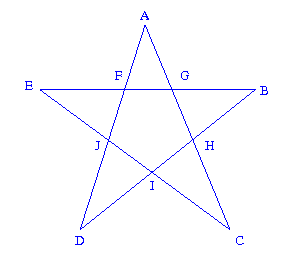
\includegraphics{figures/star}}

\vfill

}

\workbookpagebreak

\item Sketch a graph of the relation 
\[
\{ (x,y) \suchthat x,y \in \Reals \; \mbox{and} \; y > x^2 \}.
\]

\hint{Is this the region above or below the curve $y=x^2$?}

\wbvfill

\item A function $f(x)$ is said to be \index{invertible function} 
\emph{invertible} if there is another function $g(x)$ such that 
$g(f(x)) = x$ for all values of $x$.  (Usually, the inverse function,
$g(x)$ would be denoted $f^{-1}(x)$.)   Suppose a function is presented 
to you as a relation -- that is, you are just given a set of pairs.  
How can you distinguish whether the function represented by this list 
of input/output pairs is invertible?  How can you produce the inverse 
(as a set of ordered pairs)?
 
\hint{If $f$ sends $x$ to $y$, then we want $f^{-1}$ to send $y$ back to $x$.  So the inverse just has the pairs in $f$ reversed.  When is the inverse going to fail to be a function?}

\wbvfill

\workbookpagebreak

\item There is a relation known as ``has color'' which goes from the
set 
\[ F = \{orange, cherry, pumpkin, banana\} \]
to the set 
\[ C = \{orange, red, green, yellow\}. \]

\noindent  What pairs are in ``has color''?
   
\hint{Depending on your personal experience level with fruit there may be different answers.  Certainly
(orange, orange) will be one of the pairs, but (orange, green) happens too!}

\wbvfill

\end{enumerate}


%\newpage
%\renewcommand{\bibname}{References for chapter 1}
%\bibliographystyle{plain}
%\bibliography{main}

%% Emacs customization
%% 
%% Local Variables: ***
%% TeX-master: "GIAM-hw.tex" ***
%% comment-column:0 ***
%% comment-start: "%% "  ***
%% comment-end:"***" ***
%% End: ***

